\section{Opening cycles of planned links}\label{sec:cycles}

It remains to execute the plans in \Cref{prop:partition}. Regard a block as one node and map its target layer to the block containing that layer, or to a rooted sink if the target is marked rooted. Each nonsink node has exactly one outgoing edge. A component therefore reaches a rooted sink or contains one directed cycle. Additional graph intersections between layers can only help; the following argument does not need them to be recorded by this bookkeeping graph.

\begin{lemma}[One free period]\label{lem:free-period}
A block of $k$ layers and period $p$ can be joined internally, in place of its outgoing link, for cost at most $(k-1)p$. Thus this replacement leaves at least $p$ of its total budget available.
\end{lemma}

\begin{proof}
For an individual block, or any block with $k=1$, no internal addition is needed. For a collective block, \eqref{eq:sharp-band} gives
\[
f_H(t)-l_{L_*}(t)\le(k-1)p.
\]
Apply \Cref{lem:band} with $h=(k-1)p$.
\end{proof}

\begin{lemma}[A short contact on a maximal link]\label{lem:cycle-contact}
On a directed cycle of blocks, choose a block whose group's distinguished forward rotation is lexicographically greatest. If its target layer has period $q$, its planned outgoing link can be realized within its reserved budget so that the resulting connected piece contains a vertex of length at most $q$.
\end{lemma}

\begin{proof}
If the plan is an individual link, \eqref{eq:single-short} already gives the contact. For a collective plan with $k$ source layers of period $p$, put $K=kp$. Recall that $t$ is distinguished, $H=f_H(t)$, and the target record $R=[a,b)$ agrees with the source text and satisfies
\[
a\le t<H-K\le b,\qquad b-a<p+q.
\]
If any constituent layer already contains a vertex of length at most $q$, the ordinary collective link connects that vertex to the target and to all other constituents, so it suffices.

Otherwise every vertex on every constituent layer has length greater than $q$. Every forward rotation of the target's text is at most its own distinguished rotation, and hence at most the selected block's distinguished rotation. The target alignment is different from the source alignment by construction. If $b-t\ge q$, agreement on $R$ would include all $q$ positions starting at $t$, contrary to \Cref{lem:max-rotation}. Thus
\begin{equation}\label{eq:cycle-agreement}
b-t<q.
\end{equation}
Put $x=\min(t,a+K)$. We have $a\le x\le a+K$ and $x\le t<b$. If $x=t$, \eqref{eq:cycle-agreement} gives $b-x<q$. If $x=a+K<t$, then
\[
b-x=b-a-K<p+q-K\le q.
\]
Thus $[x,b)$ is a suffix of $R$ of length less than $q$.

At start $x$, every constituent layer's first end exceeds $b$, because its corresponding word has length greater than $q>b-x$. These first ends are all at most $H$: they are no greater than the top first end at $x$, which is at most its first end at $t$. Let $F=f_H(x)$. Then $b<F\le H\le b+K$. Descend from $R$ to $[x,b)$ and grow at start $x$ to $[x,F)$. This growth touches every constituent at its first end, and all intermediate words are prefixes of the actual top-layer vertex. Finish at $R+K$.

In summary, the prescribed list is
\begin{equation}\label{eq:cycle-list}
[a,b),\qquad[x,b),\qquad[x,F),\qquad[a+K,b+K).
\end{equation}
Its starts and ends are nondecreasing. Every prescribed word is in $V$, and the last equals the first in the period-$p$ source text. \Cref{lem:ordered-windows} makes it a cost-$K$ closed walk, with the short contact $[x,b)$.
\end{proof}

\begin{theorem}[Connecting the base graph]\label{thm:connection}
The base graph can be connected to $\eps$ by adding closed walks of total up cost at most $W$.
\end{theorem}

\begin{proof}
Use the group procedure of \Cref{sec:processing}. Its fulfilled requests and direct connections have already rooted the layers outside outgoing blocks within their assigned budgets. Consider the remaining functional graph.

For a cycle consisting of one block, its target layer belongs to the same block, hence to the same primitive-text group. The chosen record has a different alignment, so \eqref{eq:same-group-record} gives $\len R<p$. Replace the outgoing link by the internal joining of \Cref{lem:free-period}. The target layer, and therefore $R$, lies in this joined piece. The freed budget $p$ pays for a round trip between $R$ and $\eps$.

For a cycle of at least two blocks, choose the outgoing link in \Cref{lem:cycle-contact}; write $q$ for its target block's period. Retain that selected link, with its contact of length at most $q$. Omit the \emph{target block's} outgoing link, replacing it by internal joining. This frees $q$ by \Cref{lem:free-period}. The selected link and the omitted link are different, since the cycle has length greater than one. All other cycle links, together with the target's internal joining, connect the entire cycle into one piece. Use the freed $q$ to root the short contact. \Cref{fig:cycles} illustrates this choice of the omitted edge.

Distinct directed cycles have disjoint blocks, so these replacements do not compete for budgets. Finally execute the links leading into the rooted pieces, in increasing distance from a root or an opened cycle. Each attaches its source block using only that source's reserved budget. All layers are now rooted.

Every addition is a closed walk. The initial layer budgets sum to $W$, and each budget was used only in its assigned operation or its cycle replacement. The total added up cost is therefore at most $W$.
\end{proof}

\begin{figure}[t]
\centering
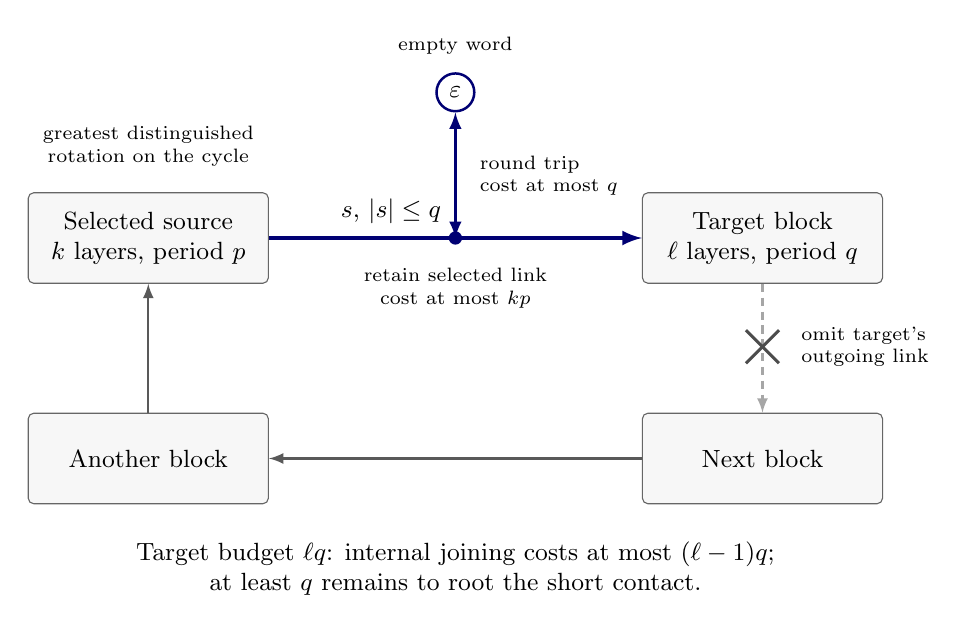
\begin{tikzpicture}[font=\small,>=latex,
  block/.style={draw=black!60,rounded corners=2pt,fill=black!3,
    minimum width=3.05cm,minimum height=1.15cm,align=center,inner sep=5pt},
  link/.style={->,draw=black!65,line width=.8pt},
  selected/.style={->,draw=blue!45!black,line width=1.4pt}]
  \node[block] (source) at (0,2.8)
    {Selected source\\$k$ layers, period $p$};
  \node[block] (target) at (7.8,2.8)
    {Target block\\$\ell$ layers, period $q$};
  \node[block] (next) at (7.8,0)
    {Next block};
  \node[block] (last) at (0,0)
    {Another block};

  \draw[selected] (source.east) -- (target.west)
    node[midway,below=7pt,align=center,font=\scriptsize]
      {retain selected link\\cost at most $kp$};
  \draw[link] (next.west) -- (last.east);
  \draw[link] (last.north) -- (source.south);

  \draw[->,draw=black!35,densely dashed,line width=.8pt]
    (target.south) -- (next.north);
  \draw[black!70,line width=1.1pt] (7.59,1.21) -- (8.01,1.63);
  \draw[black!70,line width=1.1pt] (7.59,1.63) -- (8.01,1.21);
  \node[anchor=west,align=left,font=\scriptsize] at (8.17,1.42)
    {omit target's\\outgoing link};

  \coordinate (contact) at (3.9,2.8);
  \fill[blue!45!black] (contact) circle (2.4pt);
  \node[anchor=south east,inner sep=5pt] at (contact) {$s$, $|s|\le q$};
  \node[circle,draw=blue!45!black,fill=white,line width=.9pt,
    minimum size=.48cm,inner sep=2pt] (root) at (3.9,4.65) {$\varepsilon$};
  \node[above=3pt,font=\scriptsize] at (root.north) {empty word};
  \draw[<->,draw=blue!45!black,line width=1.05pt]
    (contact) -- (root.south)
    node[midway,right=5pt,align=left,font=\scriptsize]
      {round trip\\cost at most $q$};

  \node[above=6pt,align=center,font=\scriptsize] at (source.north)
    {greatest distinguished\\rotation on the cycle};
  \node[anchor=north,align=center] at (3.9,-.93)
    {Target budget $\ell q$: internal joining costs at most $(\ell-1)q$;\\
     at least $q$ remains to root the short contact.};
\end{tikzpicture}

\caption{Opening a directed cycle of planned block links. Keep a link whose source has maximal distinguished rotation and realize it with a contact of length at most $q$, the target's period. Omit the target block's outgoing link and join that block internally, freeing $q$ to connect the contact to the empty word. Arrows between blocks represent planned dependencies, each realized by a closed walk; the dot is a contact vertex, not an extra block.}
\label{fig:cycles}
\end{figure}
